%
% trans.tex
%
% (c) 2018 Prof Dr Andreas Müller, Hochschule Rapperswil
%
\documentclass[tikz]{standalone}
\usepackage{times}
\usepackage{amsmath}
\usepackage{txfonts}
\usepackage[utf8]{inputenc}
\usepackage{graphics}
\usetikzlibrary{arrows,intersections}
\begin{document}

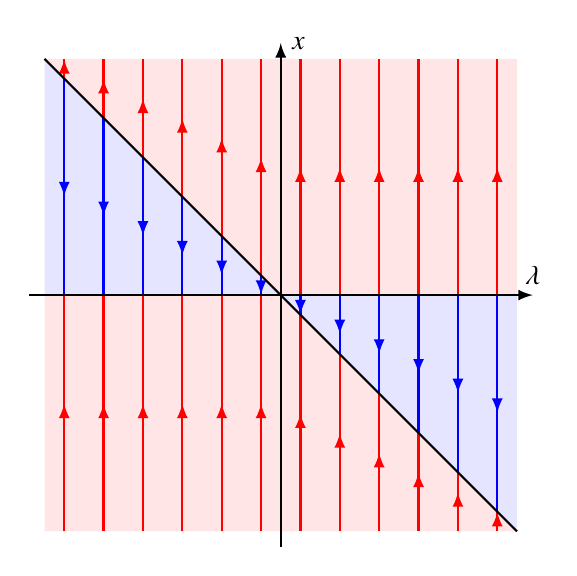
\begin{tikzpicture}[>=latex,thick]

\def\l{3}
\def\s{0.12}

\fill[color=red!10] ({-\l},0)--(0,0)--({\l},{-\l})--({-\l},{-\l})--cycle;
\fill[color=red!10] ({-\l},{\l})--(0,0)--({\l},0)--({\l},{\l})--cycle;
\fill[color=blue!10] (0,0)--({\l},{-\l})--({\l},0)--cycle;
\fill[color=blue!10] ({-\l},0)--(0,0)--({-\l},{\l})--cycle;

\pgfmathparse{-\l+0.25}
\edef\lfirst{\pgfmathresult}
\pgfmathparse{-\l+0.75}
\edef\lsecond{\pgfmathresult}
\pgfmathparse{\l-0.25}
\edef\llast{\pgfmathresult}

\foreach \x in {\lfirst,\lsecond,...,-0.25}{
	\draw[->,color=red] ({\x},{-\x})--({\x},{(\l-\x)/2+\s});
	\draw[color=red] ({\x},{(\l-\x)/2})--({\x},{\l});
	\draw[->,color=red] ({\x},{-\l})--({\x},{-\l/2+\s});
	\draw[color=red] ({\x},{-\l/2})--({\x},0);
	\draw[->,color=blue] ({\x},{-\x})--({\x},{-\x/2-\s});
	\draw[color=blue] ({\x},{-\x/2})--({\x},0);
}

\foreach \x in {0.25,0.75,...,\llast}{
	\draw[->,color=red] ({\x},{-\l})--({\x},{-(\l+\x)/2+\s});
	\draw[color=red] ({\x},{-(\l+\x)/2})--({\x},{-\x});
	\draw[->,color=red] ({\x},0)--({\x},{\l/2+\s});
	\draw[color=red] ({\x},{\l/2})--({\x},{\l});
	\draw[->,color=blue] ({\x},0)--({\x},{-\x/2-\s});
	\draw[color=blue] ({\x},{-\x/2})--({\x},{-\x});
}

\draw ({-\l},{\l})--({\l},{-\l});

\draw[->] ({-\l-0.2},0)--({\l+0.2},0) coordinate[label=$\lambda$];
\draw[->] (0,{-\l-0.2})--(0,{\l+0.2}) coordinate[label={right:$x$}];

\end{tikzpicture}

\end{document}
